\documentclass[a4paper, dvipdfmx]{jarticle}
\usepackage{rsj2011e}
\usepackage{graphicx}
\usepackage{amsmath,amssymb}
\usepackage{here}
\usepackage{booktabs}
\usepackage{url}

%余白設定
\setlength{\columnsep}{2zw}
\usepackage[top=15truemm,bottom=15truemm,left=25truemm,right=25truemm]{geometry}

\begin{document}
\title{画像システム特論発表用レジュメ}
\author{小谷岳 松下日昇}

\setlength{\baselineskip}{4.4mm}
\maketitle
\thispagestyle{empty}
\pagestyle{empty}

\section{概要}
本稿では、画像システム特論の課題として「4.ア
プリケーションを作ってみた」に取り組む。
大学院生の本文は研究である。
研究にあたり、分野の先行研究について論文を読むことが当然求められる。
これがつらい。英語読めない。
工学系研究科電気系工学専攻に所属する修士一年生にとって、輪講発表に向けて何十本と論文を読み、必死に30分の発表を行ったことは記憶に新しい(まだ終わってない人は頑張って下さい)。
論文を読む際、PCやタブレットでPDFを読むスタイルや、印刷したものにペンで書きこむスタイルなど、論文の読み方は人それぞれである。
それぞれにメリット・デメリットがあるが、本稿では特に、「論文を読む際に、印刷してペンで書きこむスタイル」の人に向けたアプリケーションを提案する。
筆者は「論文を読む際に、印刷してペンで書きこむスタイル」の人である。
このスタイルの一番のデメリットは、論文の管理が困難な点にある。
自分の書き込んだコメントなどを含めて管理しようと思うと、結局PDF上にコメントを書き直すしか手段がなく、印刷した意味が薄れる。それでも筆者は印刷物を読む方が好みである。何とかならないか。
本稿で提案するアプリケーションは、PDFを印刷し書き込んだ論文の写真画像から書き込みのみを抽出し、ホモグラフィ変換を利用してオリジナルのPDFに書き込みを反映するアプリケーションを提案し、その実装を試みる。

\section{提案手法}
% \begin{figure}[t] % 無しでもいい
%     \centering
%     \includegraphics[clip, width=\columnwidth]{fig.eps}
%     \caption{提案手法の流れ}
%     \label{fig:proposed}
% \end{figure}
%
% 提案手法の概要を説明する(図\ref{fig:proposed})。
提案手法の概要を説明する。
オリジナルの論文画像(Original)と印刷・書き込み済みの論文写真画像(Withnotes)を用意する。
二画像の特徴量をSURFに基づいて抽出し、二画像間でホモグラフィ変換の変換パラメータを推定する\cite{surf}。
推定したパラメータを用いてWithnotesを変換し、変換した画像(Converted)から書き込み(Notes)を抽出する。
最後に、NotesをOriginalに重ね合わせることで、綺麗な書き込み付き論文画像(Output)を得る。
提案手法の実装にあたっては、オープンソースのソフトウェアであるOpenCV\footnote{http://opencv.org/}を利用する。
% SURF による特徴量抽出とホモグラフィ変換の実装についてはオンラインで公開されているソースコード\footnote{http://goya813.hatenablog.com/entry/2014/11/30/180002}を参考に実装しており、工夫した点は特にない。
SURF による特徴量抽出とホモグラフィ変換の実装については、工夫した点は特にない。OpenCVが強い。
以下では、主な工夫点(何も参考にしていないという意味、新規性があるかどうかはわからない)として、書き込みの抽出アルゴリズムについて述べる。

書き込みの抽出にあたって、「Originalはグレースケール」「Notesはグレースケールではない」という強い仮定を置いている。
つまり、Convertedの各ピクセルにおいてRGBの3値が大きく偏っているものをNotesとする。
各ピクセル$p$に対し、RGB値を$(r, g, b)$とすると、書き込み抽出は以下のように表される。
\begin{eqnarray}
    v & = & \sqrt{(r-g)^2+(g-b)^2+(b-r)^2}\\
    is\_note & = & \left\{ \begin{array}{ll}
            {\rm true} & (v > threshold) \\
            {\rm false} & (else) \\
        \end{array} \right.
\end{eqnarray}
ここで、閾値は人手により経験的に設定している。
詳細な実装やライブラリのバージョン・具体的なパラメータは公開されているソースコード\footnote{https://github.com/s1-31/imagingSystem}、に記述されている。
\section{実験}
\begin{figure}[t]
    \begin{minipage}{0.33\linewidth}
        \centering
        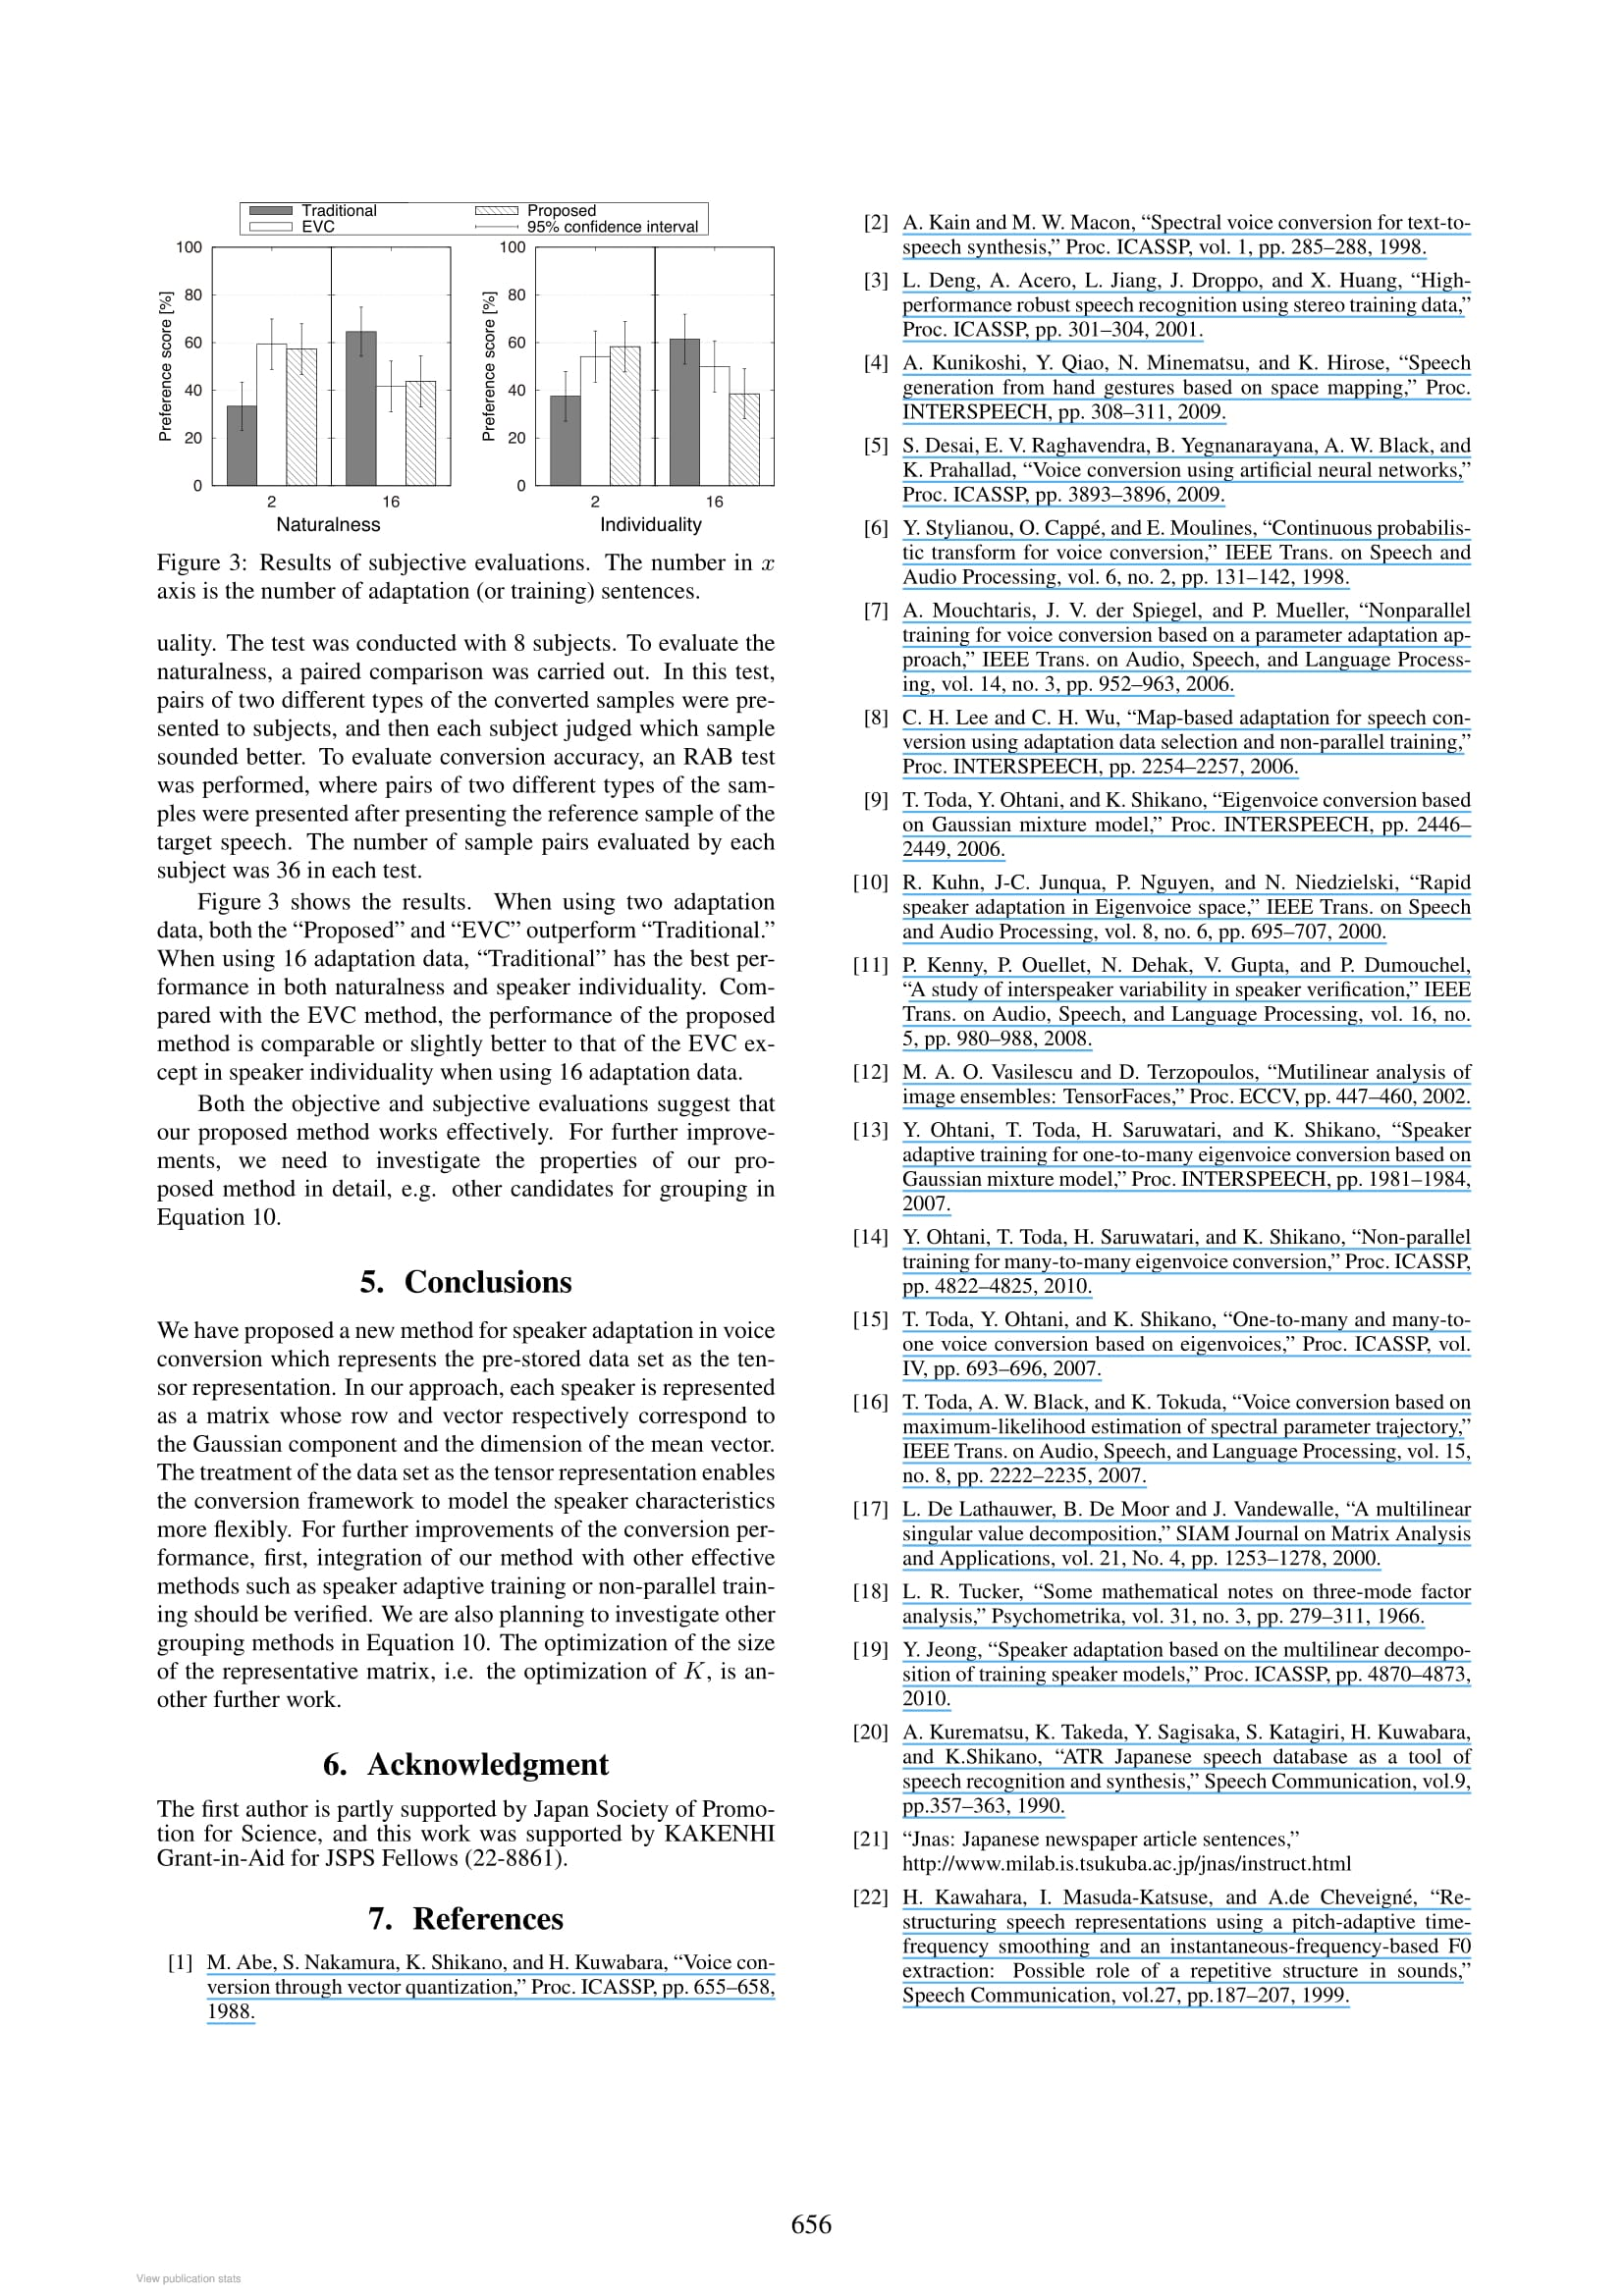
\includegraphics[clip, width=\linewidth]{fig/original.jpg}
        {\footnotesize Original}
    \end{minipage}%
    \begin{minipage}{0.33\columnwidth}
        \centering
        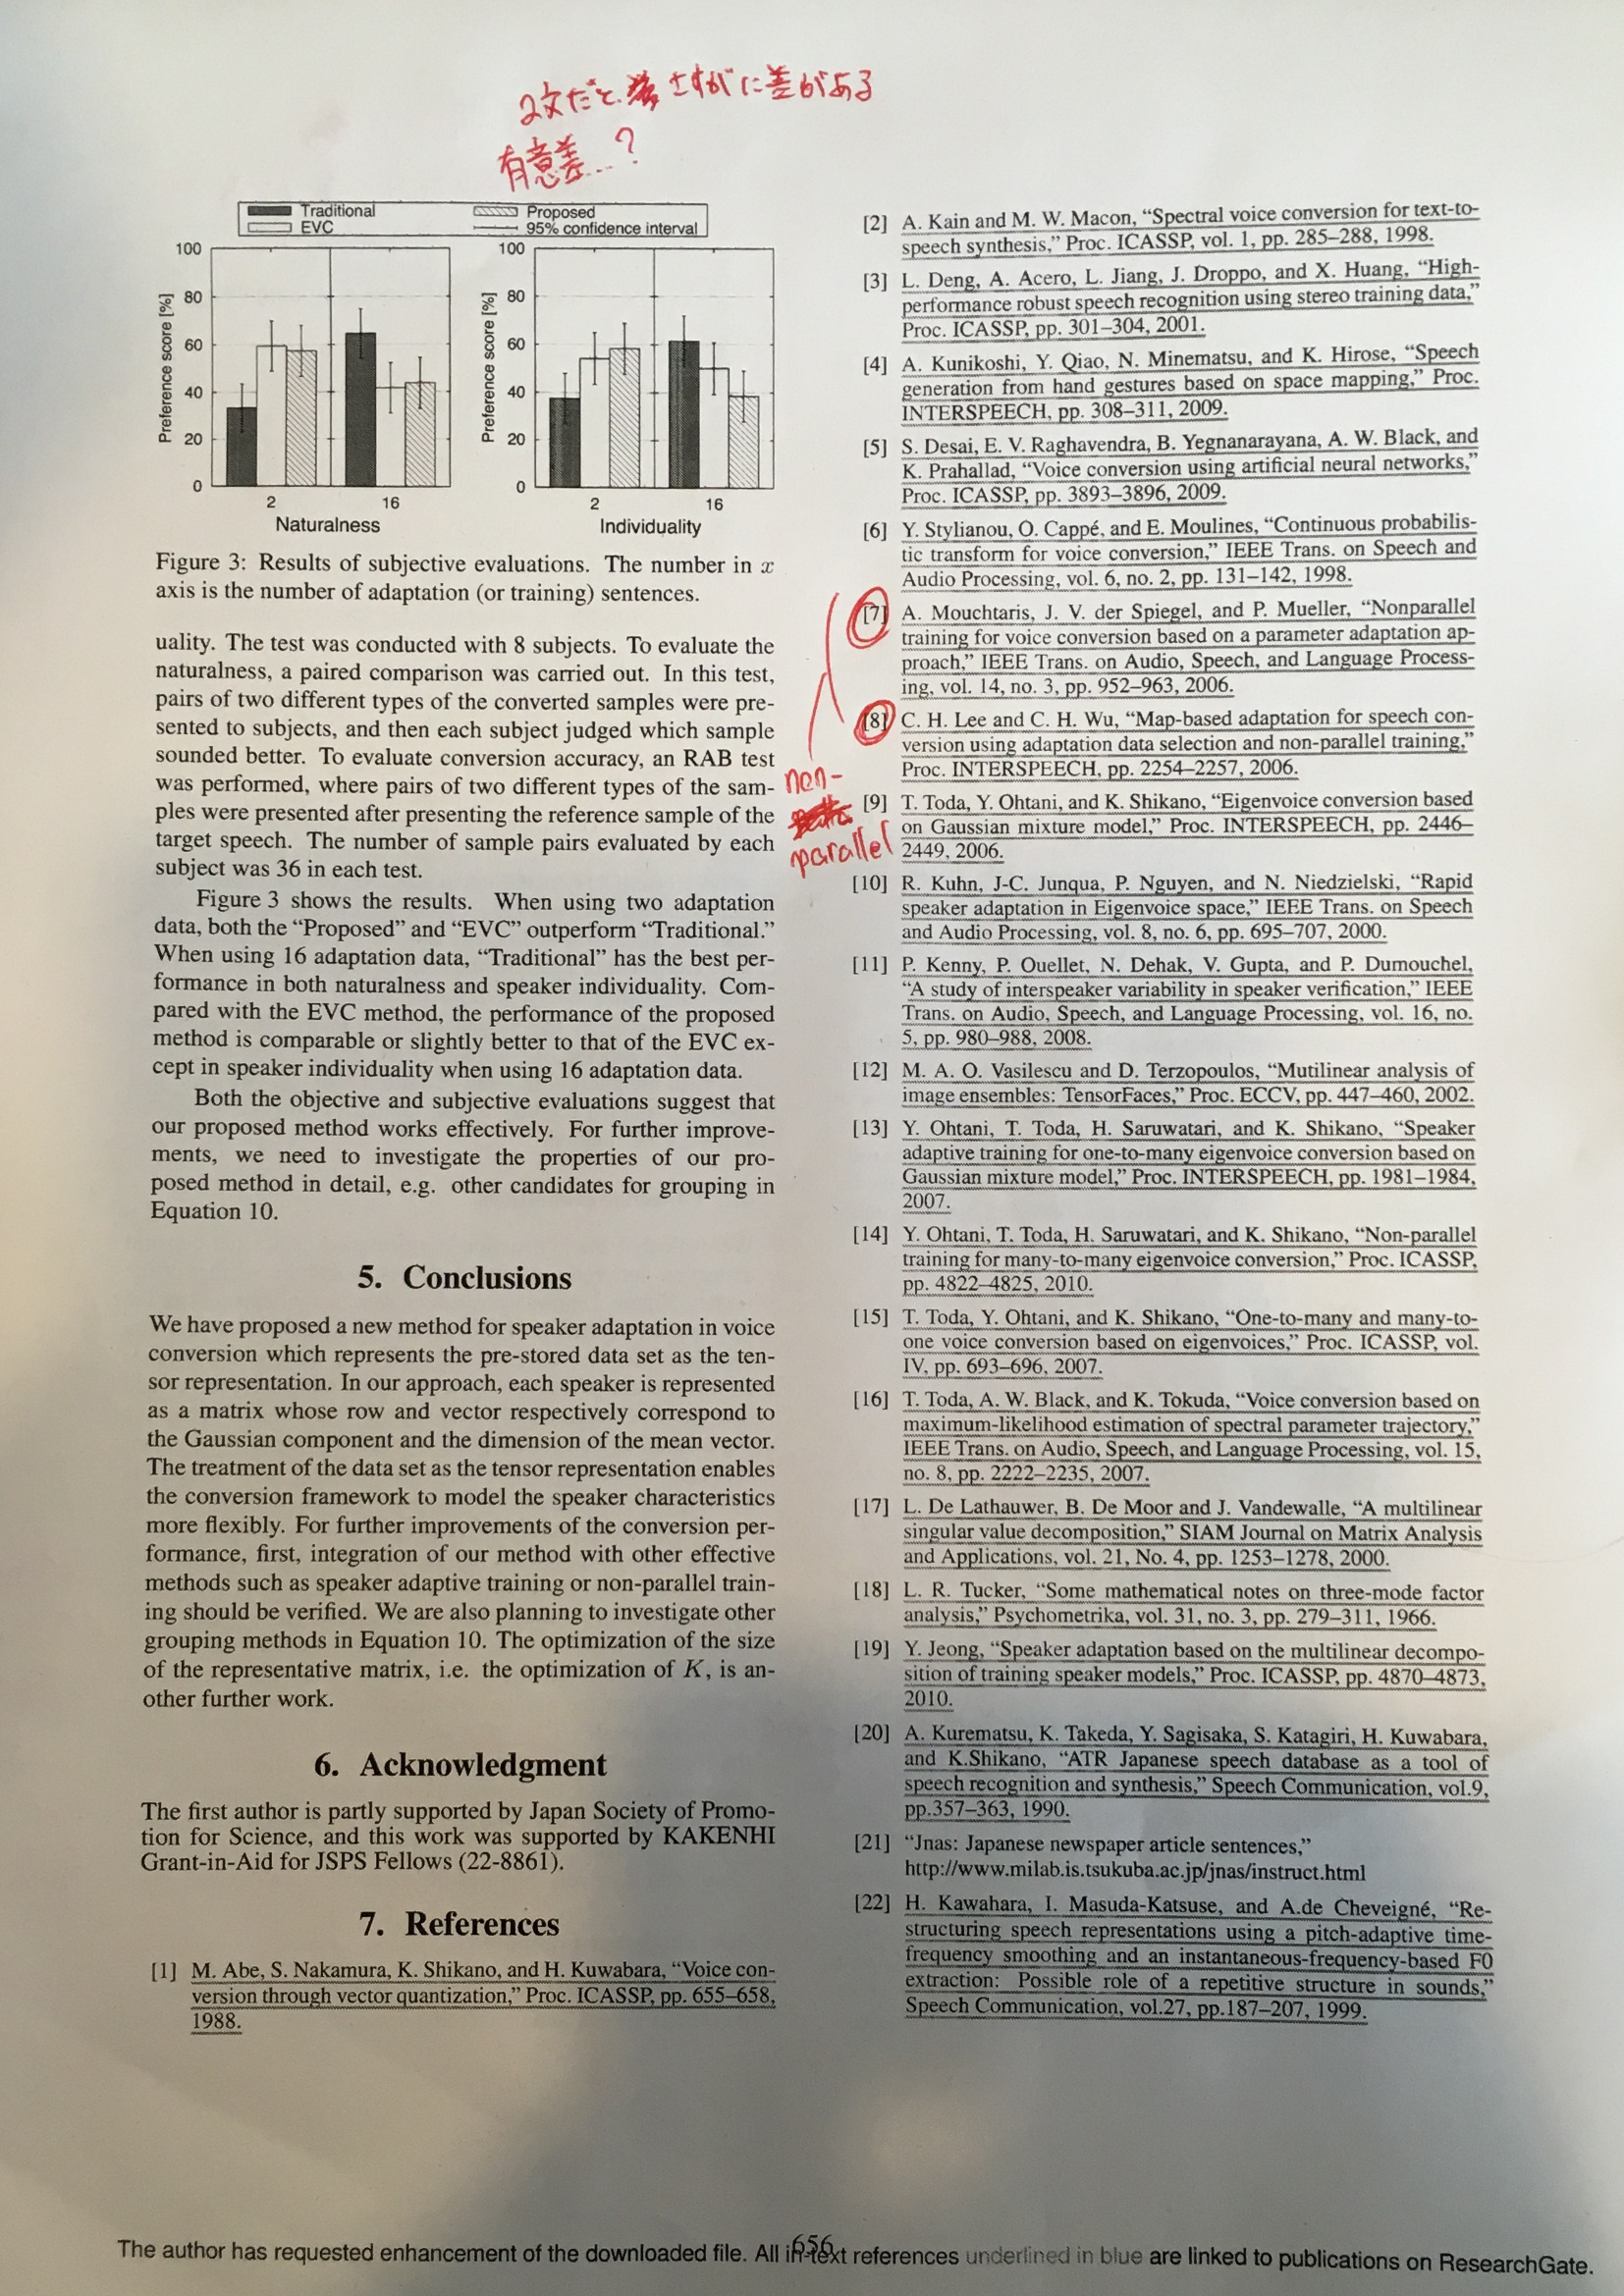
\includegraphics[clip, width=\linewidth]{fig/converted.jpg}
        {\footnotesize Converted}
    \end{minipage}%
    \begin{minipage}{0.33\columnwidth}
        \centering
        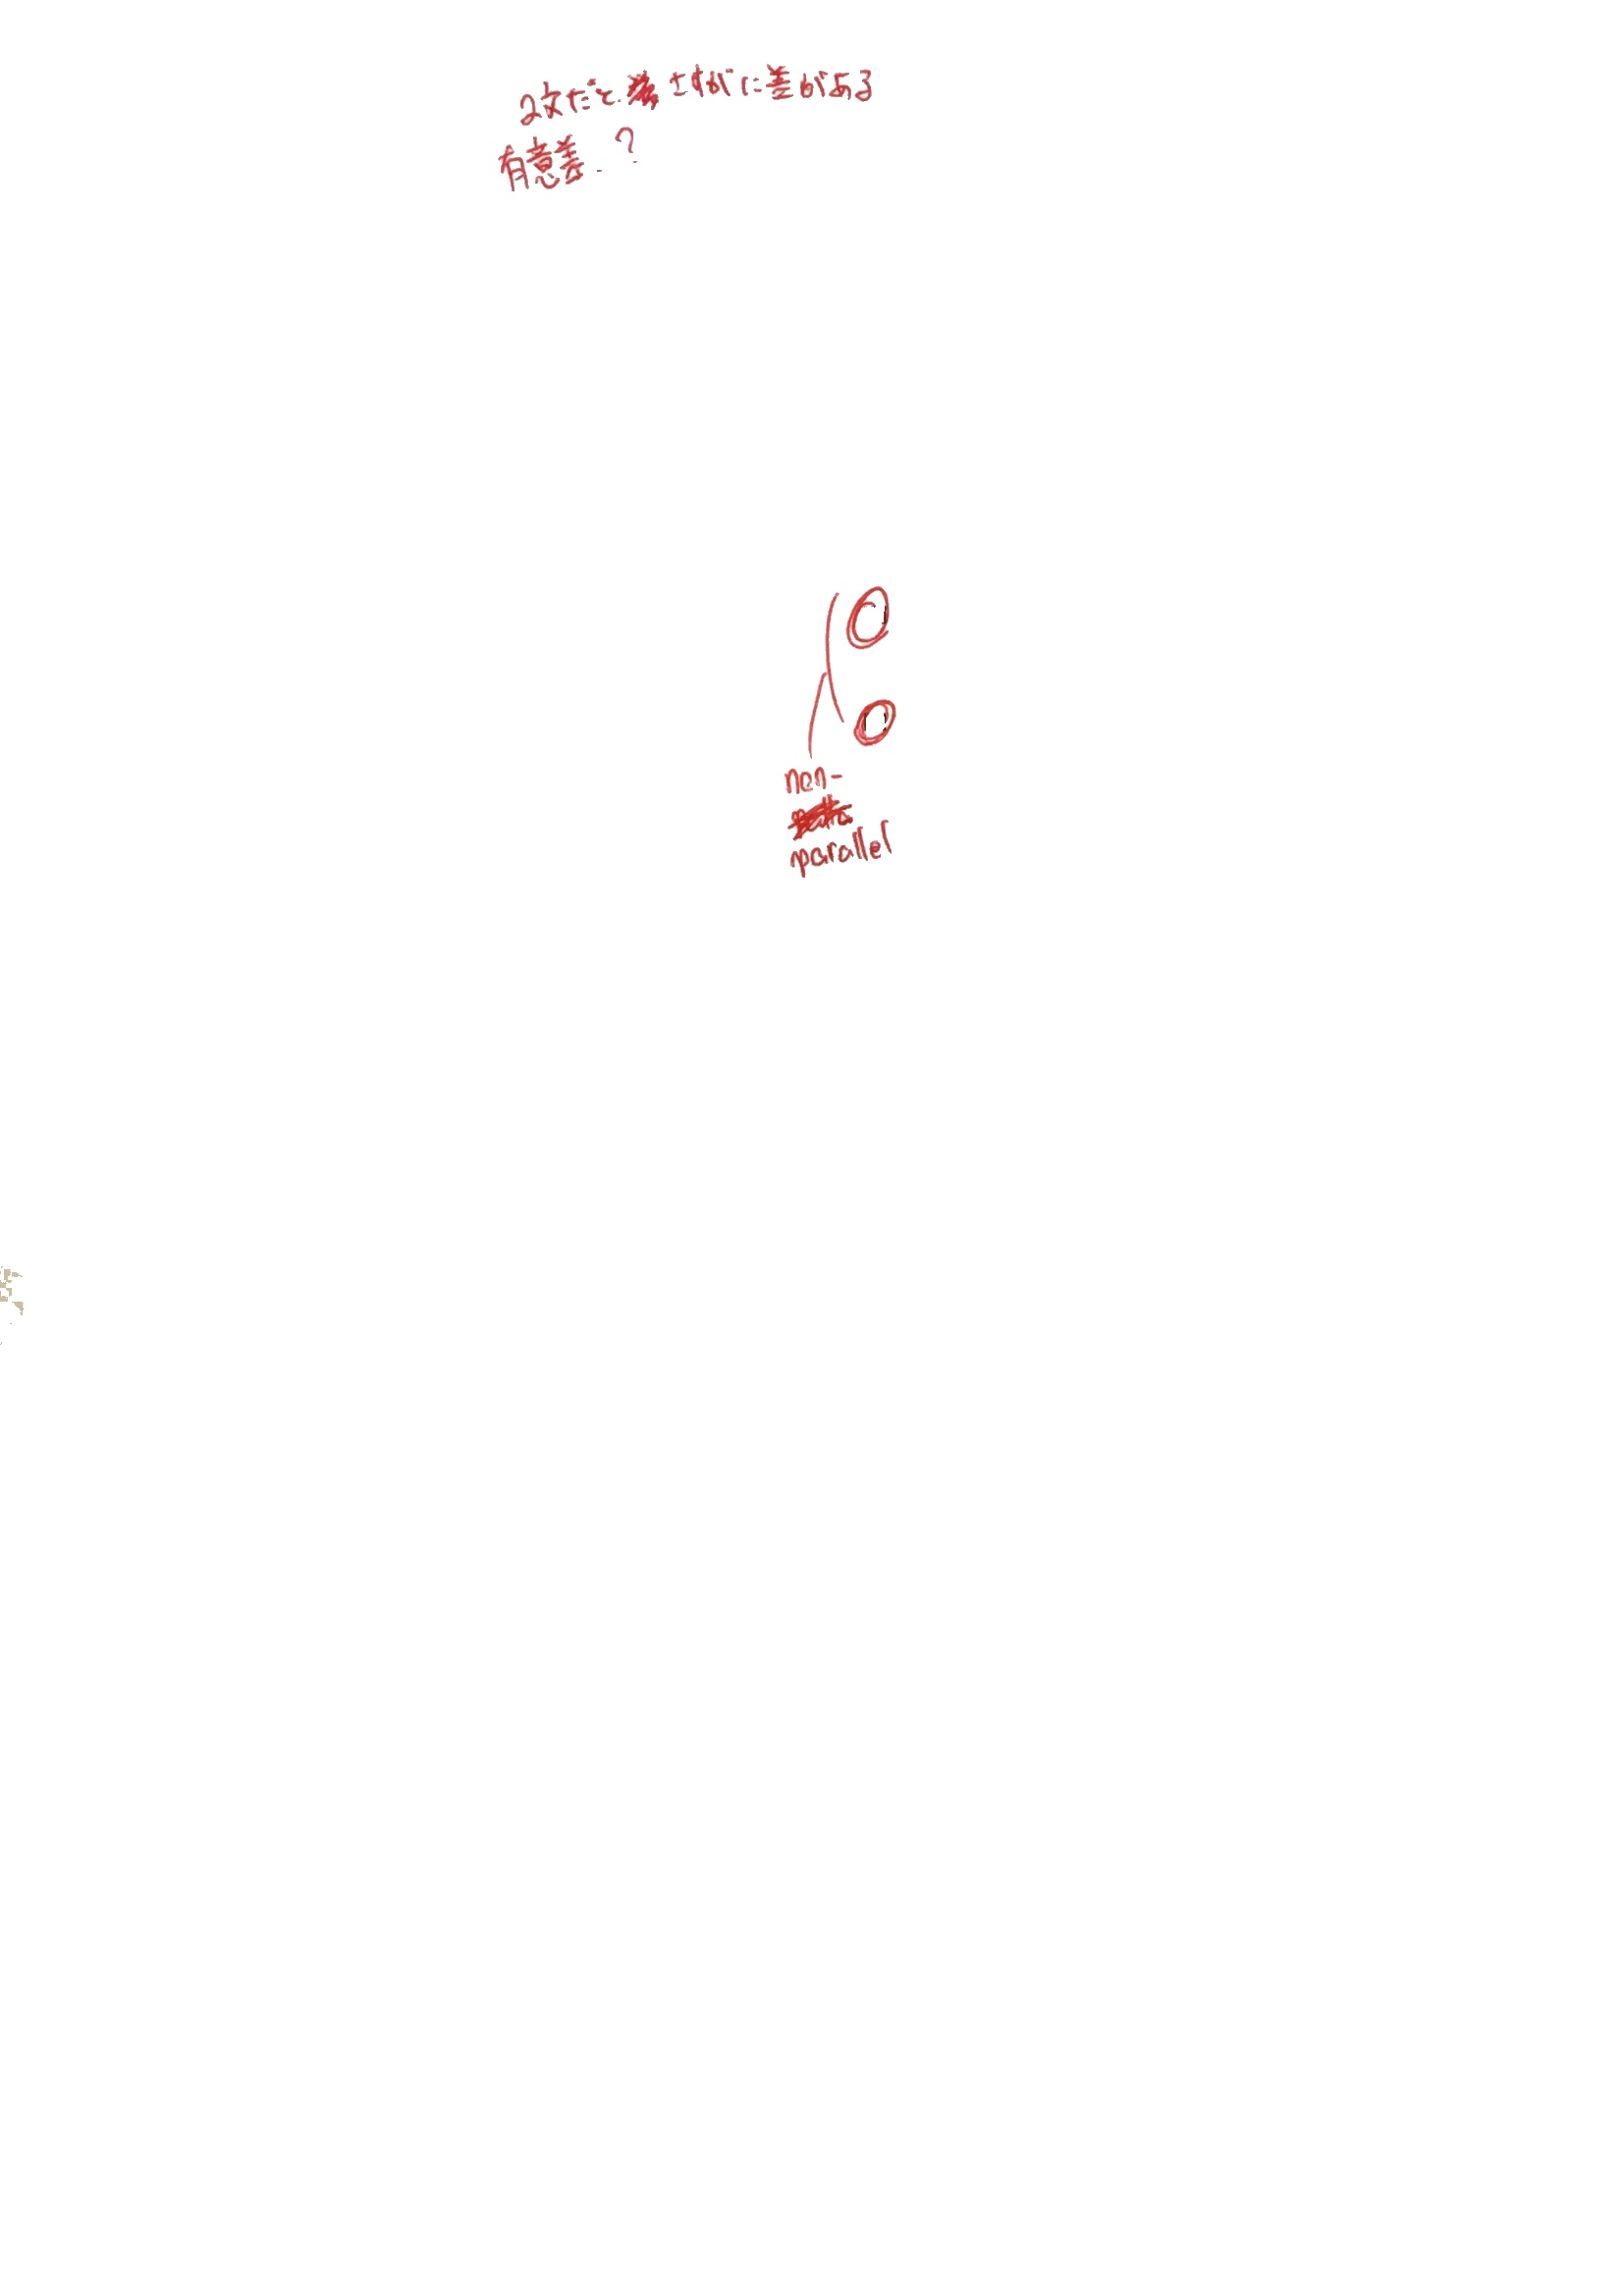
\includegraphics[clip, width=\linewidth]{fig/notes.jpg}
        {\footnotesize Notes}
    \end{minipage}\\
    \begin{minipage}{0.5\linewidth}
        \vspace{20mm}
        \centering
        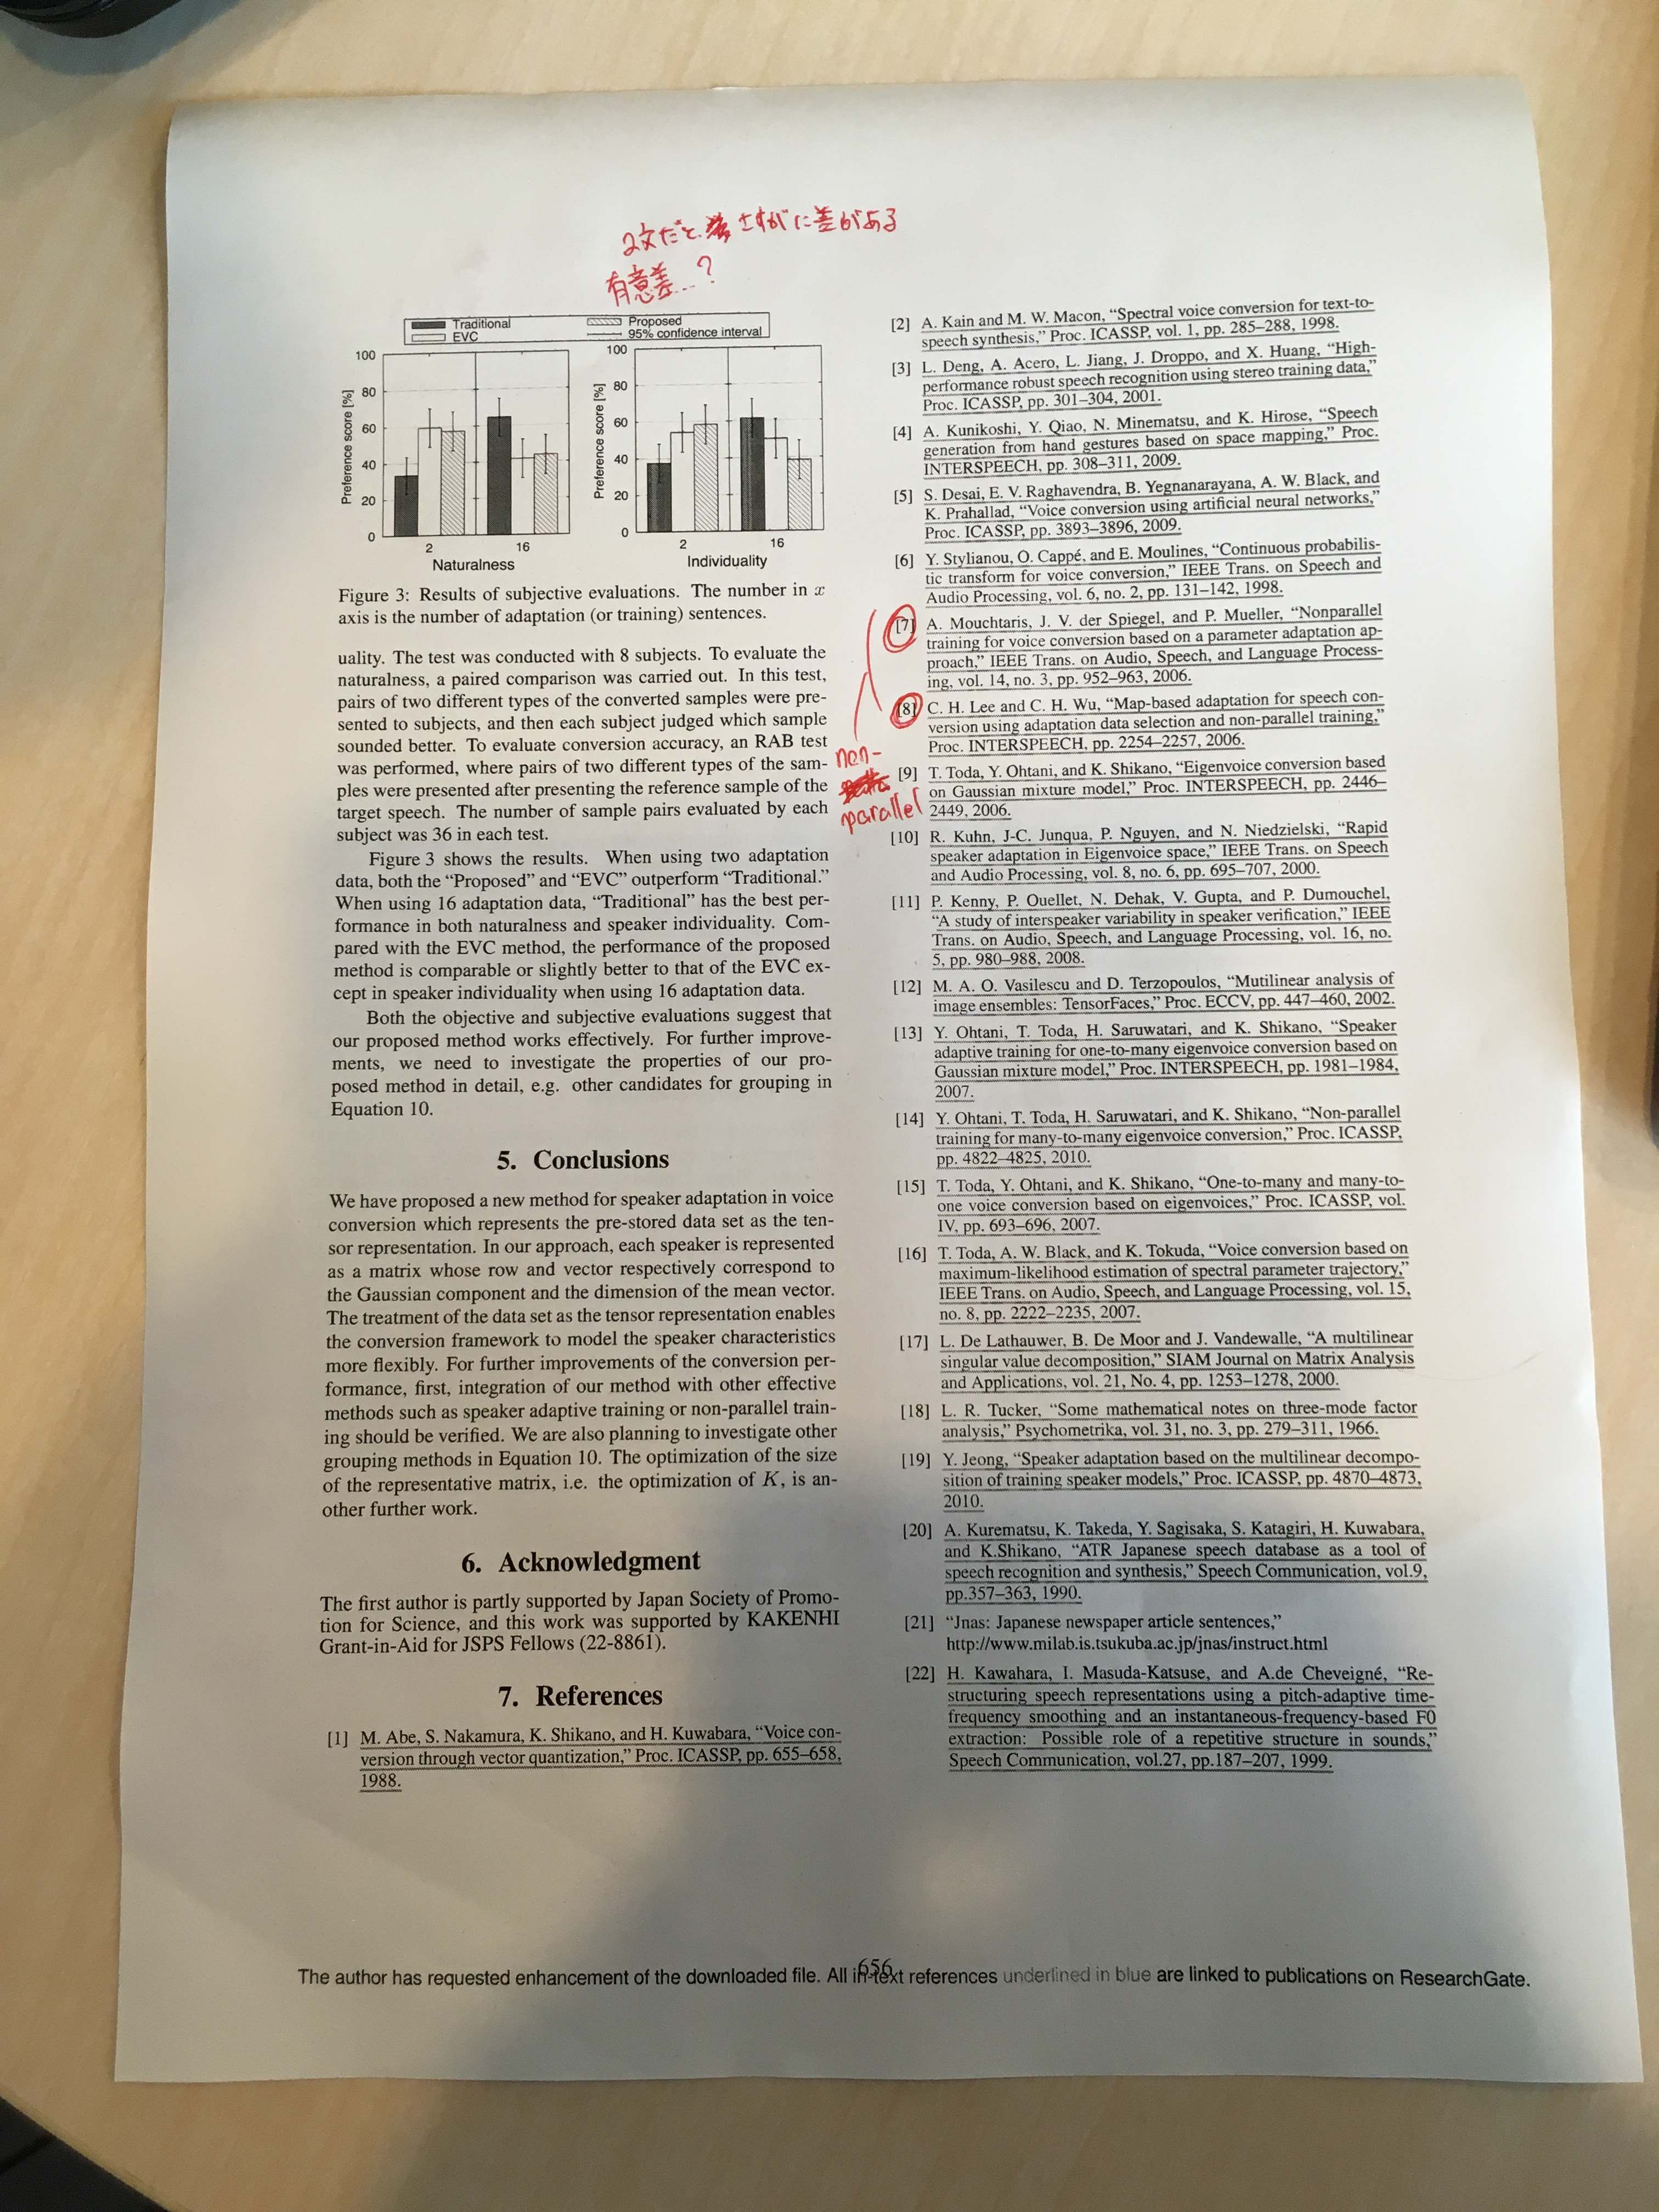
\includegraphics[clip, width=0.8\linewidth]{fig/withnotes.jpg}
        {\footnotesize Withnotes}
    \end{minipage}%
    \begin{minipage}{0.5\columnwidth}
        \centering
        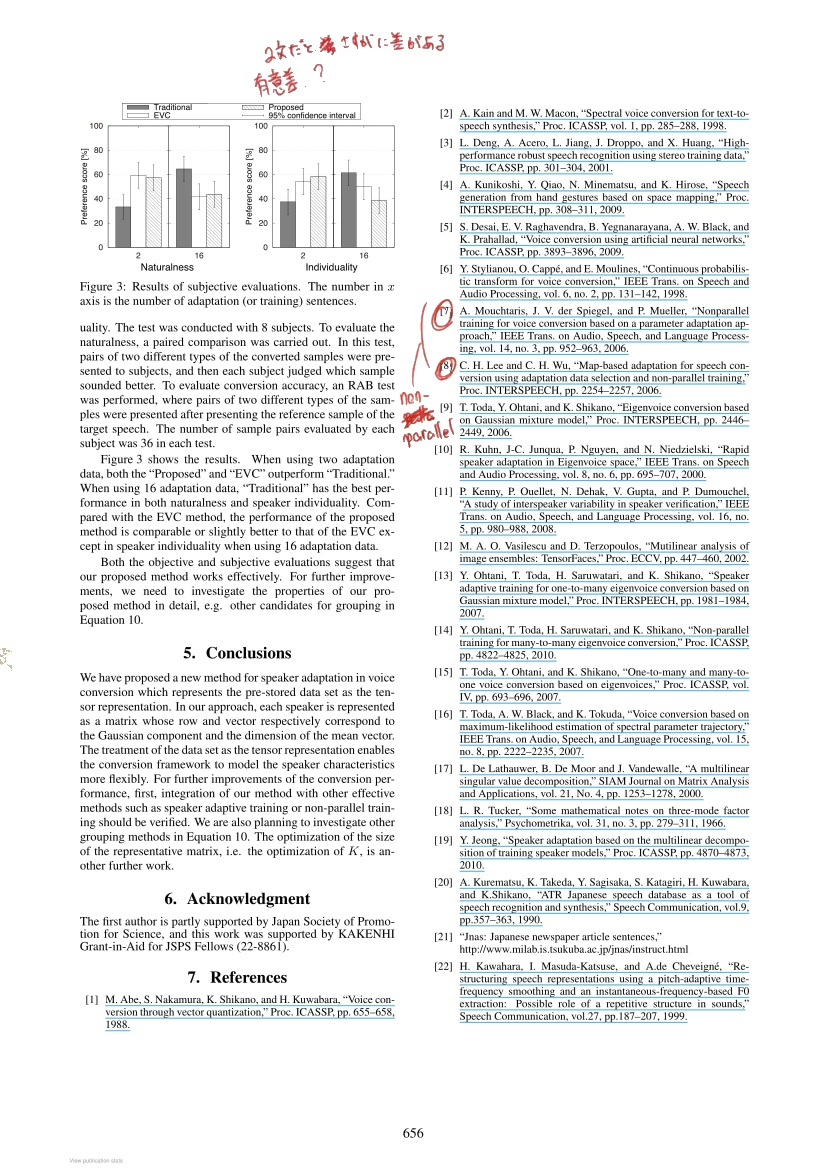
\includegraphics[clip, width=0.8\linewidth]{fig/output.jpg}
        {\footnotesize Output}
    \end{minipage}
    \caption{提案手法による書き込み抽出と合成の結果}
    \label{fig:results}
\end{figure}

実験条件について述べる。
画像として用いた論文\footnote{D. Saito \textit{et al}. \textit{Proc. Interspeech}, 2011.}について、PC上でPDFをスクリーンショットしたOriginal画像と、\textit{カメラの機種}によって書き込み付き印刷物をカメラ撮影したWithnotes画像を用意した(画像サイズ:ほげ)。
計算機としてラップトップPC(Lenovo Thinkpad E450、4コア、8Gb)を用い、一枚の画像を処理するにあたりほげ秒の実行時間を要した。

実験結果を図\ref{fig:results}に示す。
図\ref{fig:results}から、提案手法によるアプリケーションが有効に機能していることが分かる。
今後の展望としては、人手を介さない閾値設定や、複数のPDFページからの撮影された該当ページの検索が挙げられる。

\footnotesize
\begin{thebibliography}{10}

\bibitem{surf}
H. Bay \textit{et al.} : ``Speeded-Up Robust Features (SURF)'',
\textit{Computer vision and image understanding} vol.~110,  no.~3, pp.~346--359, 2008.

%%%%%%%%%%%%%%%%%%%%%%%%%%%%%%%%%%%%%%%%%%%%%%%%%%%%%%%%%%%%%%%%%%%%%%%%%%%%%%%
\end{thebibliography}
\normalsize
\end{document}
